% This document must be compiled with LuaLaTeX
\documentclass[12pt,article]{memoir}

\usepackage[letterpaper, portrait, margin=1in]{geometry}	% Standard page setup
\usepackage[USenglish]{babel}								% English typsetting conventions
\usepackage{fancyhdr}										% Headers and footers
\usepackage{graphicx}										% Additional graphics options
\usepackage{xcolor}											% Better colors
\usepackage{xpatch}											% Better macro patches
\usepackage{hyperref}										% Hyperlinks
\usepackage{fontspec}										% Custom fonts
\usepackage{tikz}											% Graphics creation
\usepackage{float}											% Figure positioning
\usepackage{tabu}											% Better tables
\usepackage[style=ieee, backend=biber]{biblatex}			% Bibliography
\usepackage[font={small,it}]{caption}						% Italic captions
\setsansfont{NeueHaasUnicaPro}
\usetikzlibrary{calc}
\usepackage[yyyymmdd]{datetime} % change date format to yyyy/mm/dd to fit ISO8601

\renewcommand{\familydefault}{\sfdefault} % set font
\renewcommand{\dateseparator}{--} % change date-seperators to - to fit ISO8601

\renewcommand\contentsname{Table of Contents}

\chapterstyle{section}
\renewcommand*{\chapnumfont}{\normalfont\HUGE\bfseries\sffamily}
\renewcommand*{\chaptitlefont}{\normalfont\HUGE\bfseries\sffamily}

\makeatletter 
% define macro for itemcode
\newcommand\itemcode[1]{\renewcommand\@itemcode{#1}}
\newcommand\@itemcode{}

% define macro for rev number
\newcommand\revnumber[1]{\renewcommand\@revnumber{#1}}
\newcommand\@revnumber{}
\makeatother

\definecolor{orbitOrange}{RGB}{250,62,0} % the ORBiT orange

\setlrmarginsandblock{2.5cm}{2.5cm}{*}
\setulmarginsandblock{2.5cm}{*}{1}
\checkandfixthelayout 

\setlength{\beforechapskip}{0cm} % reduce chapter spacing

\hypersetup{
    colorlinks,
    citecolor=black,
    filecolor=black,
    linkcolor=black,
    urlcolor=black
}

% Background swoosh
\newcommand\OrbitBackground[1]{% For a logo drawn with TikZ
	\begin{tikzpicture}[remember picture,overlay] % draw background
	\coordinate (bl) at (current page.south west);
	\coordinate (r) at (current page.east);
	\coordinate (A) at ($(bl)+(0,3cm)$);
	\coordinate (B) at ($(r)+(0,-2cm)$);
	\coordinate (C) at (current page.south east);
	\coordinate (ctrlNode) at ($(current page.south) + (0cm,1cm)$);
	\coordinate (ctrlNode2) at ($(current page.south east) + (-1cm,1cm)$);
	\fill[orbitOrange, fill opacity={#1}]
	(A) .. controls (ctrlNode) and (ctrlNode2) .. (B) -- (C) -- (bl);
	\node [white] at ($(C) + (-3cm,1cm)$) {2015-\the\year \ ORBiT@SU};
	\end{tikzpicture}
}

%**********************************************************************
% Document titles etc. defined here: (replace [] as well)
\title{OA-II VEH TAM System Design}
\author{Jinzhi Cai}
\itemcode{DR00004}
\revnumber{A02}
\date{\today}
% End of document titles etc.
%**********************************************************************

% set header style
\makeatletter
\pagestyle{fancy}
{
	\fancyheadoffset{0cm}

	\lhead{\@title \ - \@itemcode}
	\rhead{Page: \thepage }
	%\chead{\leftmark} % section name
}
\makeatother

\cfoot{\OrbitBackground{0.2}}

\begin{document}
	
\OrbitBackground{1}

\makeatletter

\includegraphics[width=\textwidth]{../Templates/logo.jpg}\\[4ex]
\begin{center}
	\bfseries \fontsize{50}{50}\selectfont  \@title \\[2ex]
	\LARGE  \@itemcode
\end{center}
\vfill
\begin{flushright}
	\LARGE Rev: \@revnumber\\
	\large \@author\\
	\large \@date\\[18ex]
\end{flushright}
\makeatother
\thispagestyle{empty}
\newpage

\tableofcontents*
\thispagestyle{fancy}
\newpage

\tableofcontents*
\clearpage

%**********************************************************************
% Everything after this is the main document. Edit below this line.

\chapter{Introduction}
\section{Scope}
This document analyzes the requirements of ORBiT Avionics System II Vehicle Electronics Telecommunication and Acquisition Module(OA-II VEH TAM) and recommend the best design approach.
\section{Purpose}
The goal of this document is use to analyze current sensor technology and come up with a design that fit the system requirements.
\section{Relevant Documents}
\begin{description}
	\item[\textbf{ER00002}]ORBiT Avionics System II Requirements
	\item[\textbf{ES00002}]ORBiT Avionics System II Architecture
	\item[\textbf{ES00003}]OA-II Vehicle Electronics (VEH) System Architecture
	\item[\textbf{DR00001}]OA-II Backplane Bus System
	\item[\textbf{DR00002}]OA-II VEH Camera System Design
\end{description}
\section{Revision History}
\begin{table}[H]
	\centering
	\begin{tabu}{r || c | c | c | c }
		Rev & Author & Approver & Changes & Date\\ \hline
		A01 & Jinzhi Cai & Jinzhi Cai & Initial draft & 2019-7-22 \\
	\end{tabu}
	\caption{Summary of Revision History}
	\label{tab:rev}
\end{table}
\newpage
\chapter{Requirement Analysis}
\section{General Requirement Analysis}
The TAM system requirements can be divided into two parts. The first part is the bridge which transfers data from a low speed parallel sensor connection to the high speed serial backplane. The second part is controls, which configure all the sensors to connect to the board and execute basic unit transformations.
\section{Bridge Requirement Analysis}
The TAM sensor unit needs to be have to bridge different data buses to the backplane data bus. The TAM sensor unit needs to support: 
\section{Control Requirement Analysis}
The TAM sensor unit needs to be able to configure the sensor to the correct state and execute basic data transformation to transfer data to real physical values. The delay should not be more than 100ms and should support up to 32 channels.
\newpage
\chapter{Current Controller Analysis}
\section{Microcontroller}
It does come with many interface options. However, it does not have a high speed interface needed for connections between other systems. It is different than the requirement, which needs a few kind of interfaces with high speed connectivity.
\section{FPGA Soft Core Processor}
A field-programmable gate array (FPGA) is an integrated circuit designed to be configured by a customer or a designer after manufacturing – hence the term "field-programmable".\cite{Cite Needed} Almost every FPGA company will have it own soft core processor. This allows the core to be easily reprogrammed, as it is formed by "logical synthesis" and allow the user to rebuild them in the FPGA chip as long as the chip has enough resources. However, the speed of this soft core processor will not be as fast as the SoC processor. Although, it is fairly easy to interface to other systems.\section{SoC FPGA}
The SoC FPGA is another kind of FPGA. The difference is the embedded, more powerful processor know as hard core processor. It helps fuse the benefit between the SoC chip and FPGA chip designs. On one hand, it allows a big system to run in the powerful hard core processor, and, at the same time, the flexibility of an FPGA chip allows a custom interface and upgradibility. However, SoC FPGAs have less logical resources compared with a classic FPGA and weak proessing power when compared with SoC which is the same cost.\newpage
\chapter{Recommand Design}
\begin{figure}[htp]
\begin{center}
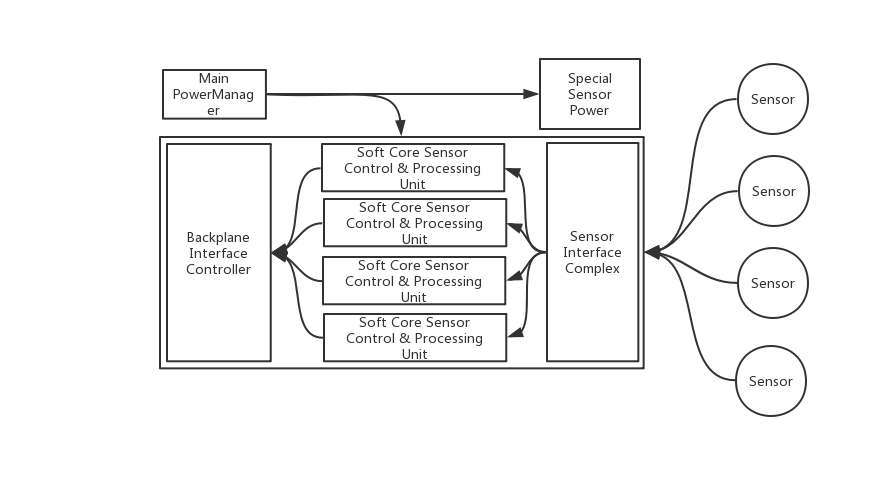
\includegraphics[width=\textwidth]{img/DR00004_FPGA.png}
 \caption{Block Diagram For TAM System}	
\end{center}
\end{figure}
% End of document
%**********************************************************************
\end{document}
